\documentclass[aps, prl, letterpaper, twocolumn, superscriptaddress, notitlepage, 10pt]{revtex4-1}
\usepackage{times}

% use these settings for a more reader-friendly version
%\documentclass[aps, pra, a4paper, 11pt, onecolumn, nofootinbib, superscriptaddress, tightenlines, notitlepage, longbibliography]{revtex4-1}

%------------------------------------------------------------------------------------------------------------%
% Packages
%------------------------------------------------------------------------------------------------------------%

\usepackage{xcolor}
\usepackage{amsmath,amsfonts,amssymb}
\usepackage{graphicx}
\usepackage[caption=false]{subfig}
\usepackage{enumerate}
\usepackage{mathrsfs}


%\usepackage{epstopdf} % to include .eps graphics files with pdfLaTeX

\usepackage[pdfpagelabels,pdftex,bookmarks,breaklinks]{hyperref}
\definecolor{darkblue}{RGB}{0,0,127} % choose colors
\definecolor{darkgreen}{RGB}{0,150,0}
\hypersetup{colorlinks, linkcolor=darkblue, citecolor=darkgreen, filecolor=red, urlcolor=blue}
\hypersetup{pdfauthor={Simon Burton, Courtney G. Brell, Steven T. Flammia}}
\hypersetup{pdftitle={Classical Simulation of Quantum Error Correction in a Fibonacci Anyon Code}}

\usepackage[normalem]{ulem}

%------------------------------------------------------------------------------------------------------------%
\begin{document}

\title{Supplemental material for ``Classical Simulation of Quantum Error Correction in a Fibonacci Anyon Code''}

\author{Simon Burton}
\affiliation{Centre for Engineered Quantum Systems, School of Physics, 
The University of Sydney, Sydney, Australia}
\author{Courtney G.\ Brell}
\affiliation{Institut f\"{u}r Theoretische Physik, Leibniz Universit\"{a}t Hannover, 
Appelstra\ss{}e 2, 30167 Hannover, Germany}
\author{Steven T.\ Flammia}
\affiliation{Centre for Engineered Quantum Systems, School of Physics, 
The University of Sydney, Sydney, Australia}

\date{\today}

\maketitle

% CUT HERE

%------------------------------------------------------------------------------------------------------------%
% Macros
%------------------------------------------------------------------------------------------------------------%

\newcommand{\Eref}[1]{Eq.~(\ref{#1})}
\newcommand{\Fref}[1]{Fig.~\ref{#1}}
\newcommand{\Aref}[1]{Appendix~\ref{#1}}

\newcommand{\e}{\mathrm{e}}
\newcommand{\vac}{\mathbb{I}}

\newcommand{\ket}[1]{|{#1}\rangle}
\newcommand{\expect}[1]{\langle{#1}\rangle}
\newcommand{\bra}[1]{\langle{#1}|}
\newcommand{\ketbra}[2]{\ket{#1}\!\bra{#2}}
\newcommand{\braket}[2]{\langle{#1}|{#2}\rangle}
\newcommand{\proj}[1]{\ketbra{#1}{#1}}

\newcommand{\cggb}[1]{\textcolor{blue}{#1}}
\newcommand{\simon}[1]{\textcolor{red}{#1}}
\newcommand{\stf}[1]{\textcolor{green}{#1}}


\newcommand{\F}{\mathscr{H}} % H or F ?
\newcommand{\C}{\mathbb{C}}
\newcommand{\R}{\mathbb{R}}
\newcommand{\A}{\mathcal{A}}
\newcommand{\Hom}{{\mathrm{Hom}}}

\newcommand{\subsub}[1]{{\bf #1}}

%------------------------------------------------------------------------------------------------------------%

% CUT HERE
\onecolumngrid
\appendix
% CUT HERE



%The goal here is to describe the algorithm for
%computing charge contained in regions built from 
%arbitrary collections of tiles.
%To do this we first describe our approach
%to topological quantum field theory,
%then we discuss the data structure 
%(combinatorial curve diagrams) and the algorithm
%that operates on these structures.

%We give an informal introduction to
%anyonic topological quantum
%field theory in $(2+1)$-dimensions.
%See \cite{beverland2014} for a similar treatment.
%Note that these theories give rise to
%\emph{doubled} anyonic charges, and so
%the Fibonacci example in the main text simulates
%one half of such a system. % MEH!

%
% ~~~~~~~~~~~~~~~~~~~~~~~~~~~~~~~~~~~~~~~~~~~~~~~~~~~~~~~~~~~~~~~~~~~~~~~~~~~~
%

%\section{A TQFT warmup}
%
%In two spacial dimensions, particle exchange is
%captured by the braid group.
%World lines of such particles 
%become tangled (braided) in $(2+1)$-dimensions.
%For example, three particle statistics is captured
%by the braid group on three strands $B_3.$
%This group is generated by elements $\sigma_1$
%and $\sigma_2$ which we represent pictorially as:
%\begin{center}
%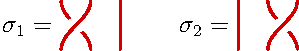
\includegraphics[]{pic-braid-group.pdf}
%\end{center}
%
%These pictures make clear how the group
%multiplication works, for example:
%\begin{center}
%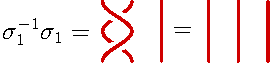
\includegraphics[]{pic-braid-group-1.pdf}
%\end{center}
%\begin{center}
%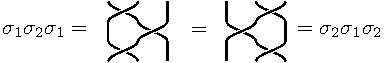
\includegraphics[]{pic-braid-relation.pdf}
%\end{center}
%
%
%These diagrams are to be understood up to
%continuous deformation of the ambient space.
%That is, we allow the ambient $(2+1)$-dimensional
%space with these worldlines subtracted to be continuously
%deformed.
%At the top and bottom of this space is 
%a $2$-dimensional space (a disc) with holes in it.
%Such a closed disc with $n$ holes we denote as $D_n.$
%So this is how we arrive at modelling the system as
%a disc with holes in it.
%The observables of the system measure charge within
%a region bounded by a directed closed curve.
%\begin{center}
%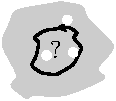
\includegraphics[]{pic-observable.pdf}
%\end{center}
%
%The defining feature of an Abelian anyon theory
%is that the state is completely determined once
%we measure the charge of each hole.
%In the language of the toric code (homology),
%logical operators (1-chains)
%cancel where they overlap
%with opposite orientation:
%\begin{center}
%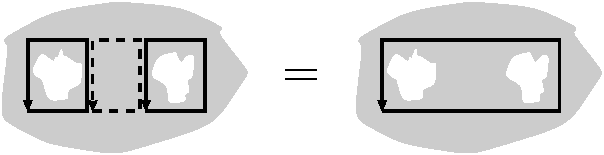
\includegraphics[width=0.4\columnwidth]{pic-abelian.pdf}
%\end{center}
%
%This is not at all the case in general;
%for non-Abelian theories there can be extra
%degrees of freedom associated with these
%observables. For example, in
%a system supporting Fibonacci anyons,
%we can have two Fibonacci anyons with total
%charge either vacuum or Fibonacci:
%\begin{center}
%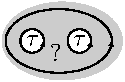
\includegraphics[]{pic-fusion.pdf}
%\end{center}
%so the state space of two fibonacci anyons
%is $2$-dimensional.
%Such a space associated with observing total charge
%of multiple anyons is called the \emph{fusion} space
%of those charges.
%
%These observables satisfy various relations,
%but in particular, non-overlapping observables commute.
%So if we nest a maximal set of these observables together
%we can pin-down a basis for the fusion space.
%Such a nesting is tree-like, and if we confuse the distinction
%between holes and observables, this gives rise to the
%fusion tree notation.
%\begin{center}
%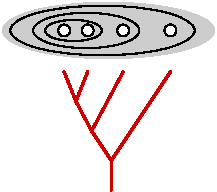
\includegraphics[]{pic-tree-0.pdf}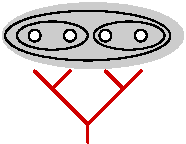
\includegraphics[]{pic-tree-1.pdf}
%\end{center}
%
%Given a disc with $n$ holes, we define the \emph{mapping
%class group} $MCG(D_n)$ as the group of topological
%symmetries (homeomorphisms) of the space $D_n,$
%modulo continuous deformations (isotopy).
%Such symmetries we require to fix the boundary
%of the disc, but not necessarily to fix the holes.
%Elements $f\in MCG(D_n)$ will also act on anything that
%resides in $D_n.$ 
%In particular, if we draw a line
%connecting the holes:
%\begin{center}
%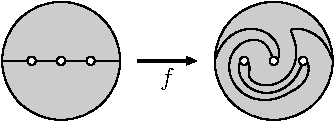
\includegraphics[]{pic-twist.pdf}
%\end{center}
%
%Such an embedding $c : [0, 1] \to D$ with $c(0), c(1) \in \partial D$
%and touching all holes in $D_n$ we call a \emph{curve diagram}~\cite{Dehornoy2002},
%(or just a \emph{curve} when the context is clear).
%
%We can think of braids acting on states in a Schrodinger picture,
%or alternatively, elements of the mapping class group acting on
%observables in a Heisenberg picture:
%\begin{center}
%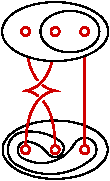
\includegraphics[]{pic-interaction.pdf}
%\end{center}
%
%We would hope that the groups $B_n$ and $MCG(D_n)$ are
%isomorphic, and this is indeed the case~\cite{Kassel2010}.
%One can see this as follows. Dragging the space $D_n$ along
%a braid creates a deformation, the end point of which is a
%homeomorphism in $MCG(D_n).$ Going the other direction,
%given $f\in MCG(D_n)$ and a curve diagram $c,$ we think of
%pulling the ends of $f\circ c$, thereby moving (braiding) the holes,
%until we are back at the original curve $c.$
%
%%This discussion makes it clear we have picked out a
%%specific curve $c$ that we use as a reference point for
%%other curves. 
%
%The importance of this isomorphism: the simulation
%algorithm calculates outcomes of observations. This
%boils down to a change of basis, to one that includes
%the required observable.
%$F$-moves allow us to re-associate observables along
%a curve diagram. The mapping class group acts
%transitively on curve diagrams (\emph{why??}).

%
% ~~~~~~~~~~~~~~~~~~~~~~~~~~~~~~~~~~~~~~~~~~~~~~~~~~~~~~~~~~~~~~~~~~~~~~~~~~~~
%

We consider the theory of two-dimensional topologically ordered systems
with anyonic excitations.
There are two main approaches to defining these,
one being more algebraic and the other more topological.

The algebraic side is known to mathematicians as the study of braided
tensor categories, or more specifically, modular tensor categories.
This algebraic language appears to be more commonly used 
in the physics literature~\cite{Kitaev2006}.
Such algebraic calculations can be interpreted as
manipulations of string diagrams~\cite{Baez2010},
or \emph{skeins}, which begins to hint at
how knot theory and topology comes into play.

Building from the other direction, one starts with
a topological space (of low dimension) and attempts
to extract a combinatorial or algebraic description of how this
space can be built from joining smaller (simpler) pieces together.
This is perhaps more difficult to grapple with.
These topologically rooted constructs are known as modular functors, 
or the closely related topological quantum field theories (TQFT's).
%The much older study of Homology also extracts algebraic
%information out of topological spaces, but 

That these two approaches (algebraic versus topological)
meet is one of the great
miracles of modern mathematics and physics.

%There is somewhat of a gap between the algebraic/skein-theoretic
%approach and the topological approach

Modular functors can be constructed from skein theory.
In the physics literature, 
this appears as skeins mysteriously growing out of manifolds \cite{Pfeifer2012},
or as motivated by renormalization group considerations \cite{Levin2005}.
A further physical motivation is this: if a skein 
is supposed to correspond to the $(2+1)$-dimensional
world-lines of particles
as in the Schr\"{o}dinger picture,
modular functors would
correspond to the algebra of observables, as in
a Heisenberg picture.

In the physics literature, modular functors are
explicitly used in \cite{Freedman2002, Freedman2002simulation}.
Also, \cite{Beverland2014} and \cite{Kitaev2006topo}
use the language of modular functors but they call them TQFT's.
This is in fact reasonable because a modular functor can be
seen as (part of) a TQFT, but is quite confusing to the
novice who attempts to delve into the mathematical literature.

The definition of a modular functor appears to
be well motivated physically.
Unfortunately, there are many such definitions
in the mathematical literature 
\cite{Walker1991,Turaev1994,Bakalov2001,Tillmann1998}.
According to \cite{Bartlett2015} section 1.2 and 1.3,
there are many open questions involved in 
rigorously establishing the connection between these different axiomatizations.
%In particular, what physicists call anyon theory,
%and mathematicians call a modular tensor category,
Furthermore, the concept of modular tensor category 
has not been established to correspond exactly
(bijectively) to any of these modular functor variants. 
We try not to concern ourselves too much with these details, 
but merely note these facts as a warning to the reader
who may go searching for the ``one true formulation'' of
topological quantum field theory.

Of the many variants of modular functor found in the literature,
one important distinction to be made is
the way anyons are labeled.
In the mathematical works \cite{Turaev1994, Bakalov2001, Tillmann1998} 
we see that anyons are allowed to have superpositions
of charge states. 
However, in this work we restrict anyons to have
definite charge states, as in \cite{Walker1991,Freedman2002simulation,Beverland2014}. 
This seems to be motivated physically as such configurations
would be more stable \simon{citation?}.

One of the goals of this work is to sketch how a 
braided tensor category arises from a modular functor.
In the mathematical literature,
this is covered in \cite{Turaev1994,Tillmann1998,Bakalov2001}
but as we just noted they use a different formulation for a
modular functor.
%The much more ambitious task of deriving a modular
%functor from a braided tensor category is 

%Turaev derives a ribbon category
%from his definition of a modular functor, but this
%definition is different to the one given here 
%and is not known to be equivalent.
%Our definition is based on \cite{Walker1991},
%Walker \cite{Walker1991}
%(and others \cite{Bakalov2001}) perform the much more
%difficult task of deriving a modular functor from
%an appropriate braided tensor category,
%but do not seem to say much about going in the other direction.

%As in algebraic topology, we wish to extract
%algebraic information about topological objects.
%This can be viewed as a kind of representation theory
%of topological objects: diffeomorphisms of surfaces.

\begin{quotation}
``People these days have a tendency 
to actually define a subfactor as being some kind of
tensor category.
But these guys [subfactors] are the algebras of observables
of your physical system, and if you want to
ignore them and throw them out then you strongly
risk throwing out the baby with the bathwater.''
- Vaughan Jones~\cite{Jones2015}
\end{quotation}

\section{The Braid Group}

We consider world-lines of particles in two spacial dimensions.
Here we show three particles undergoing some exchange and then
returning to the original location:
\begin{center}
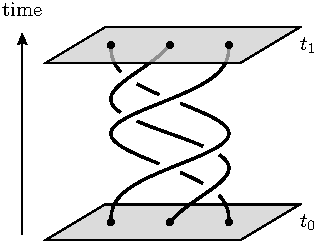
\includegraphics[]{pic-braid-worldlines.pdf}
\end{center}
Note that if we allow the particles to move in one extra
dimension then we can untangle these braided world lines.
The question is, how has the wavefunction of the system
changed from $t_0$ to $t_1$?

Examining the structure of these processes more closely,
we see that we can compose them by sequentially performing
two such braids, one after the other:
\begin{center}
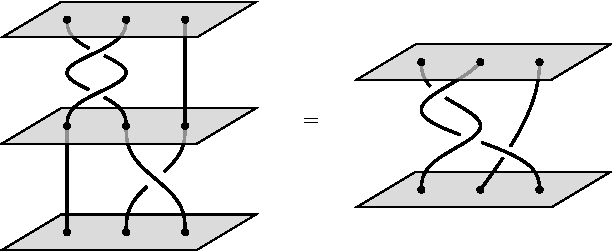
\includegraphics[]{pic-braid-compose.pdf}
\end{center}
And, by ``reversing time'', we can undo the effect of
any braid:
\begin{center}
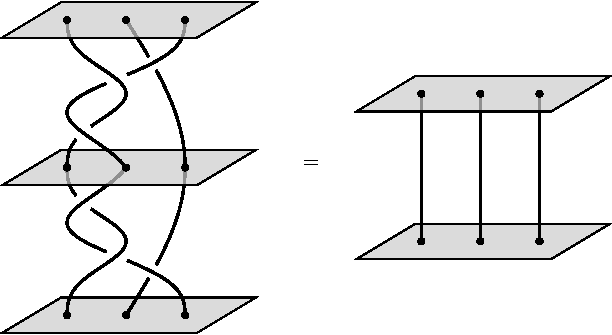
\includegraphics[]{pic-braid-inverse.pdf}
\end{center}
This means we have a group, known as the \emph{braid group.}
For $n$ particle worldlines we denote this group as $B_n.$

%The \emph{braid group} on $n$ strands is denoted $B_n.$
This group can also be described purely algebraically.
$B_n$ has $n-1$ generators $\sigma_1,..,\sigma_{n-1}$ that satisfy
the following two relations:
\begin{align*}
    \sigma_i \sigma_j &= \sigma_j \sigma_i \ \ \ \mbox{for}\ \ |i-j|>1,\\
    \sigma_i \sigma_{i+1} \sigma_i &= \sigma_{i+1} \sigma_i \sigma_{i+1} \ \ \ \mbox{for}\ \ 1\le i \le n-2.
\end{align*}

The easiest way to understand these relations is to consider the
geometric braids corresponing to the $\sigma_i.$
\begin{center}
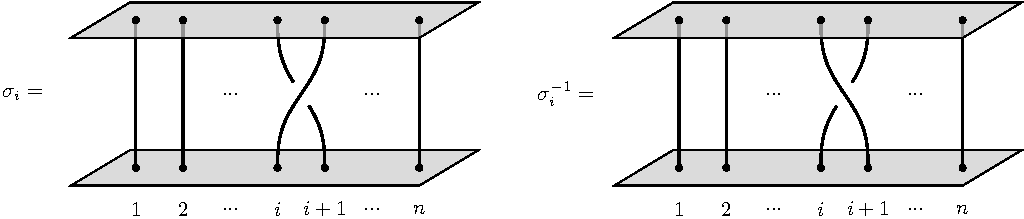
\includegraphics[]{pic-braid-sigma.pdf}
\end{center}
Now we see why 
$\sigma_i \sigma_j = \sigma_j \sigma_i \ \ \ \mbox{for}\ \ |i-j|>1,$
because the two braids are operating on disjoint strands.
To understand the second relation we draw:
\begin{center}
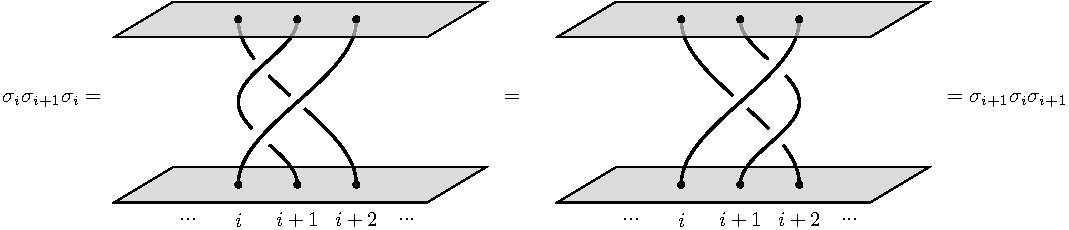
\includegraphics[]{pic-braid-YB.pdf}
\end{center}

\section{Modular Functors}

We list the axioms for a 
\emph{2-dimensional unitary topological modular functor}.
 % abbreviated as \emph{MF}.
%There are quite alot of details that we leave out,
%%For the details of this construction, see
%see
%\cite{Turaev1994}, \cite{Walker1991} or \cite{Bakalov2001}.
%For a more pedestrian treatment, see \cite{Freedman2002simulation} or \cite{Beverland2014}.

For our purposes a \emph{surface} will be a compact
oriented $2$-dimensional differentiable manifold with boundary. % smooth or topological ?
We will not require surfaces to be connected.
%Each boundary component is oriented (either explicitly or
%otherwise by using the orientation of the manifold)
By a \emph{hole} of $M$ we mean a component of its boundary. % $\partial M$.
Each hole will inherit the manifold orientation,
contain a distinguished \emph{base point},
and be labeled with
%an element from a finite set $\mathbb{A}=\{1, a, b, c ...\}.$
an element from a (fixed) finite set $\A.$
This is the set of ``anyon labels'', and comes
equiped with a vacuum element $\vac$ 
and an involution $\ \widehat{}\ $ such that $\widehat{\vac}=\vac.$
The involution maps an anyon label to the ``antiparticle'' label.

We will mostly be concerned with planar such
surfaces, that is, a \emph{disc} with holes removed from the
interior.
\cggb{Do we actually restrict to considering only such surfaces?}
\simon{Only when we get to standard surfaces and POPs...}
%Such surfaces will be given a counterclockwise 
%orientation, which induces a clockwise orientation on
%any \emph{interior} hole and a counterclockwise orientation
%on the \emph{exterior} hole.
Such surfaces will be given a clockwise 
orientation, which induces a counterclockwise orientation on
any \emph{interior} hole and a clockwise orientation
on the \emph{exterior} hole.
\begin{center}
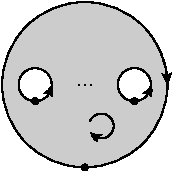
\includegraphics[]{pic-disc.pdf}
\end{center}
Although it helps to draw such a surface as a disc with holes,
we stress that there is no real distinction to be made between
interior holes and the exterior hole.
That is, 
a disc with $n$ interior holes is (equivalent to) a sphere with $n+1$ holes.
We merely take advantage of the fact that a sphere with at least one hole
can be flattened onto the page by ``choosing'' one of the holes to
serve as the exterior hole.

By a \emph{map of surfaces} $f:M\to N$ we mean 
a diffeomorphism that preserves
manifold orientation, hole labels, and base points.
\cggb{If we require that the map preserves base points and so on, are we restricting to maps between manifolds with the same number of holes?}
\simon{Yes, a diffeomorphism is also a homeomorphism, so these manifolds are
topologically equivalent.}
Note that we also deal with maps of various other objects
(vector spaces, sets, etc.)
but a map of surfaces will have these specific
requirements.

%By an \emph{isotopy} of $f:M\to N$ we mean a 
%map $g:M\to N$
%that is a continuos deformation of $f.$
Two maps $f:M\to N$ and $f':M\to N$
will be called \emph{isotopic}
when one is a continuous deformation of the other.
In detail,
we have a continuously
parametrized family of maps $f_t:M\to N$ for $t\in [0, 1]$
such that $f_0=f,\ f_1=f'$
and the restriction of $f_t$ to the 
set of marked points $X\subset\partial M$ is constant:
$f_t|_{X} = f|_{X}$ for $t\in [0, 1].$
%and the restriction of $f_t$ to the boundary is constant:
%$f_t|_{\partial M} = f|_{\partial M}$ for $t\in [0, 1].$
Such a family $\{f_t\}_{t\in [0,1]}$ is called an \emph{isotopy}
of $f.$
This is an equivalence relation on maps $M\to N$, and the equivalence
class of $f$ under isotopy is called the \emph{isotopy class} of $f.$

A \emph{modular functor} $\F$ associates to every
surface $M$ a finite dimensional complex
vector space $\F(M)$, called the \emph{fusion space} of $M$.
For each map $f:M\to N$
The modular functor associates a
unitary transformation $\F(f) : \F(M)\to\F(N)$
that only depends on the isotopy class of $f.$
Functoriality requires that $\F$
respect composition of maps.

We have the following axioms for $\F.$

{\bf Unit axioms.}
The fusion space of an empty surface is one dimensional, 
$\F(\phi) \cong \C.$ % preserves the identity of tensor
\cggb{Does a modular functor have to be over $\C$?}
\simon{No, mathematicians do this over any ring $k.$}
For $M_a$ a disc with boundary label $a$ we have
$\F(M_\vac)\cong \C$ and 
$\F(M_a)\cong 0$ for $a\ne \vac.$
For an annulus $M_{a,b}$ with boundary labels
$a, b$ we have
$\F(M_{a,\widehat{a}})\cong \C$ and 
$\F(M_{a,b})\cong 0$ for $a\ne \widehat{b}.$

{\bf Monoidal axiom.}
The disjoint union of two surfaces $M$ and $N$ 
is associated with
the tensor product of fusion spaces:
$$
    \F(M\amalg N) \cong \F(M)\otimes \F(N).
$$
This is natural from the point of view of quantum
physics, where the Hilbert space of two disjoint
systems is the tensor product of the space for
each system.

{\bf Gluing axiom.}
Denote a surface $M$ with (at least) two holes
labeled $a, b$ as $M_{a,b}$. 
If we constrain $b=\widehat{a}$ 
then we may \emph{glue} these two holes together
to form a new surface $N$.
%Let $N$ be the surface obtained from $M$ by gluing
%these two holes together.
%By this we mean there is a homeomorphism from one
To construct $N$ we choose a diffeomorphism from one
hole to the other that maps base point to base point 
and reverses orientation.
Identifying the two holes along this diffeomorphism
gives the glued surface $N$.
(There is a slight technicality in ensuring that $N$ is
then differentiable, but we will gloss over this detail.)
%Gluing must reverse the orientation of the two holes
%as well as identifying their base points.
The fusion space of $M_{a,\widehat{a}}$ then embeds unitarily in the fusion
space of $N$.
Moreover, there is an isomorphism called
a \emph{gluing map}:
$$
    \bigoplus_{a\in\A} \F(M_{a,\widehat{a}}) \xrightarrow{\cong} \F(N).
$$
\simon{say something about isotopy of gluing}

{\bf Unitarity axiom.}
Reversing the orientation of the surface $M$
to form $\overline{M}$ we get the dual of the fusion space:
$\F(\overline{M})=\F(M)^*.$
\simon{i don't think we use this for anything}

\subsub{Compatibility axioms.}
%We have left out various compatibility requirements of the axioms.
Loosely put, we require that the above operations play nicely together,
and commute with maps of surfaces.
For example,
a sequence of gluing operations 
applied to a surface can
be performed regardless of the order (gluing is associative)
and we require the various gluing maps for these operations to similarly agree.
For another example, we require $\F$ to respect that gluing
commutes with disjoint union.
%performing a gluing on $M$ and then forming $M\amalg N$
%produces the same surface as forming the disjoint union and
%then gluing the 
\cggb{I guess we should try to keep a consistent level of precision, and so probably be more explicit here.}
\simon{I agree it is a bit jarring to suddenly switch to being more informal...}

\subsub{Observables.}
The seam along which gluing occurs can be associated
with an observable as follows.
We take a gluing map $g$ and projectors $P_a$ onto the
summands in the above direct sum:
$$
    P_a: \bigoplus_{b\in\A} \F(M_{b,\widehat{b}}) \to \F(M_{a,\widehat{a}}).
$$
then the observable will be the set of operators 
$\{P_a g^{-1}\}_{a\in\A}.$
For each $a\in A$
we call the image of $P_a$ 
a \emph{charge sector} for that observable.
Note that in the glued surface $N$ the seam has no
preferred orientation (or base point).
If we choose an orientation 
for the seam this corresponds to choosing one of the
two boundary components in the original surface $M_{a,\widehat{a}}.$
If these boundary components come from disconnected components of 
$M_{a,\widehat{a}}$ the seam cuts $N$ into two pieces and the
orientation chooses an \emph{interior:}
following the orientation around the seam presents
the interior to the left.
%The projectors associated to each cuff commute.
%Non-overlapping observables commute.

%We intentionally confuse the definition of an observable as
%a set of operators 
%%$\{P_a g^{-1}\}_{a\in\A}$
%and the associated seam along which gluing occurs.
%%observable as the simple closed curve 
We intentionally confuse the distinction between an
observable as a set of operators,
and the associated seam along which gluing occurs.
Any simple closed curve within the interior of $M$
can serve as the seam along which gluing occurs...
If we now take $M$ to be an arbitrary surface, and $\gamma$ an
observable on $M,$
we can write $M$ as the gluing of another surface $N$...
\simon{XXX}

\subsub{Consequences of axioms.}
A common operation is to glue two separate surfaces.
We can do this by first taking disjoint union (tensoring
the fusion spaces)
and then gluing.
Here we show this process applied to two surfaces $M$ and $N$. 
\begin{center}
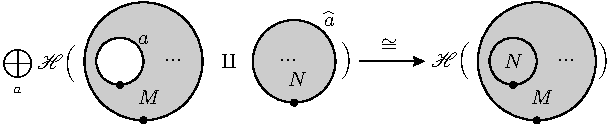
\includegraphics[]{pic-glue.pdf}
\end{center}
We display the surface $N$ with the $\widehat{a}$
boundary on the outside, 
to show more clearly how $N$ fits into $M$.
In the glued surface we
indicate the placement of $M$ and $N$ and the seam
along which gluing occurred,
as well as the identification of base points.

We note two other consequences of the axioms.
A hole of $M$ labeled with $\vac$ can be replaced with a disk (by gluing)
and this does not change the fusion space of $M.$
That is, a hole that carries no charge can be ``filled-in''.
And, the dimensionality of the fusion space of a torus is the
cardinality of $\A.$
This can be seen by gluing one end
of an annulus (cylinder) to the other.

\subsub{Fusion.}
When a surface can be presented as the gluing of
two separate surfaces, we have projectors onto the
fusion space of either glued surface:
\begin{center}
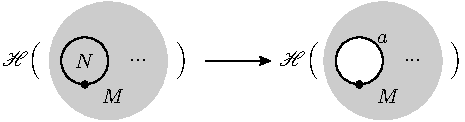
\includegraphics[]{pic-fuse.pdf}
\end{center}
In this case, we define 
the operation of \emph{fusion} to replace the interior
of an observable by a single hole.
This is an operation on the manifold itself,
and we will only do this when the interior piece is a
disc with zero or more holes.

%
%We are thinking of the holes as modelling particles
%known as \emph{anyons}.
%We have defined a collection of observables.
%We think of these as measuring the total charge of the
%anyons within a simple closed curve.
%The measurement process associated to these observables
%we call \emph{fusion}.
%When the observable is understood,
%we call this fusion of anyons.
%Such a measurement applies a projector to a state in
%some fusion space $\F(M),$ and furthermore, we modify
%the manifold $M$ by excising the interior of the observable
%to produce another manifold $N.$
%This gives a state in the fusion space $\F(N).$

%\subsub{Pair-of-pants.}
\subsub{F-move.}
The fusion space of the disc and annulus are
specified by the axioms, and we define the fusion
space of the disc with two holes, or \emph{pair-of-pants} as:
\begin{center}
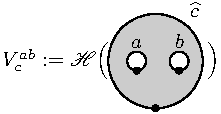
\includegraphics[]{pic-pop.pdf}
\end{center}

The \emph{$F$-move}
is constructed from two applications of a
gluing map as follows:
\begin{center}
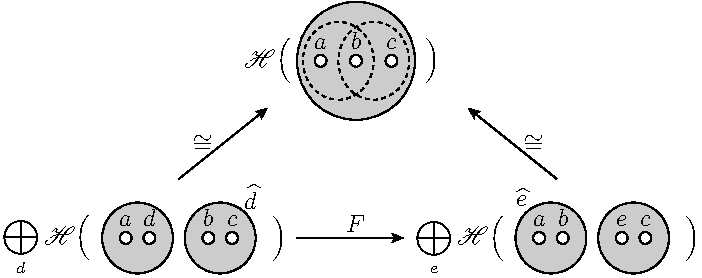
\includegraphics[]{pic-glue-fmove.pdf}
\end{center}
\cggb{Is it easy to show that such an F-move can be guaranteed to exist and be unique for a given modular functor?}
\simon{An F-move *is* two applications of a gluing map (where one is reversed).. these maps are given in the axioms. There's no trickery involved.}
Here we have shown a surface $M^{abc}_d$ with 
four labeled boundary components, as well as two separate
ways of gluing pairs-of-pants to get $M^{abc}_d.$
We can also write this out in terms of the fusion spaces of pair-of-pants:
$$
    F^{abc}_d : \bigoplus_{x\in\A} V^{ab}_{\widehat{x}}\otimes V^{xc}_d 
        \to \bigoplus_{y\in\A} V^{ay}_d\otimes V^{bc}_{\widehat{y}}.
$$
\simon{tensor with identity to extend this map under gluing}

\subsub{POP decomposition.}
%The reverse process of cutting a surface up
%into pair-of-pants induces a direct sum decomposition
%of the fusion space.
Given a manifold $M$ which is
a disc with at two or more holes, 
we show how to present $M$ as the gluing of various
pair-of-pants. Such an arangement will be termed a \emph{POP decomposition.}
(We refer to \cite{Ivanov2001} for more details on this construction,
and \cite{Ghrist2014} for a leisurely description of Morse theory.)
This will yield a decomposition of $\F(M)$ into a direct
sum of fusion spaces of pair-of-pants. % $V_{ab}^c$'s.
%The pair-of-pants can be found using Morse theory.
%We proceed using Morse theory.
%Note that we need $M$ to be a differentiable manifold for
%this to work.
The key idea is to choose a ``height'' function $h:M\to\R$
with some specific properties that allow us to
cut the manifold up along level sets of $h.$
First, we need that critical points of $h$ are isolated.
This is the defining condition for $h$ to be a \emph{Morse function}.
%Choose a Morse function (a generic ``height'' function) $h:M\to\R$
Also, we need that $h$ is constant on $\partial M,$
and the values of $h$ at different critical points are distinct.
Now choose a sequence of non-critical values $a_1<a_2<...<a_n$ in $\R$
such that every interval $[a_{i-1}, a_i]$ 
contains exactly one critical value of $h$ and the image
of $h$ lies within $[a_1, a_n].$
%cuts the manifold into pieces $f^{-1}[a,b]$.
Each component of $h^{-1}([a_{i-1}, a_i])$ is then either
an annulus, a disc, or a pair-of-pants depending on the index of (any)
critical point it contains.
We then re-glue any annuli or discs until there are no more of these
and we have only pair-of-pants. 
% note: we may still get annuli in a *component* of the pre-image.
\begin{center}
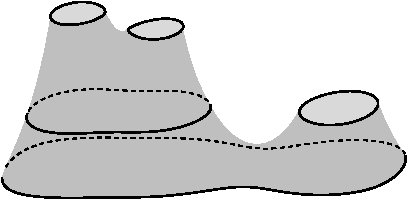
\includegraphics[]{pic-pants.pdf}\ \ \ \ \ \ \ \ 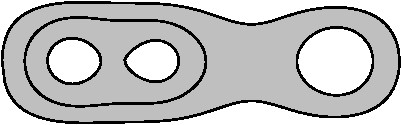
\includegraphics[]{pic-pants-1.pdf}
\end{center}

Clearly such a POP decomposition is not unique,
and the goal here is to understand how to switch between decompositions,
and in particular, given an observable $\gamma$,
and a given POP decomposition, find a sequence
of ``moves'' such that $\gamma$ is in the resulting POP
decomposition:
\begin{center}
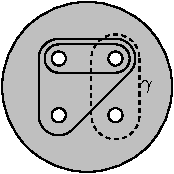
\includegraphics[]{pic-refactor.pdf}
\end{center}

One way to achieve this is via Cerf theory, which is the theory
of how one may deform Morse functions into other Morse functions
and the kind of transitions involved in their critical point structure.
This was the approach used in \cite{Freedman2002simulation}.
In this work we use a simpler method,
which is essentially the same as \emph{skein theory.}
%Read on to find out how this works!
This is the \emph{refactoring theorem}.

\subsub{Dehn twist.}
Consider a surface $M_{a,\widehat{a}}$
with two boundary components, $a$ and $\widehat{a}.$
Let $f$ be a map $M_{a,\widehat{a}}\to M_{a,\widehat{a}}$
which performs a clockwise $2\pi$ full-twist or \emph{Dehn twist}.
Here we show the action of $f$ by highlighting the
equator of the annulus:
%line between the base points:
\begin{center}
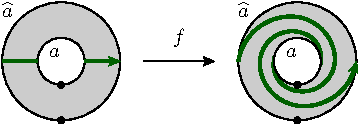
\includegraphics[]{pic-dehn-twist.pdf}
\end{center}
We define the 
induced map on fusion spaces as $\theta_a := \F(f).$
Because $\F(M_{a,\widehat{a}})$ is one-dimensional
this will be multiplication by a complex number which we also
write as $\theta_a.$

If we now take $M$ to be an arbitrary surface, and $\gamma$ an
observable on $M,$ we can consider a neighbourhood of $\gamma$
which will be an annulus, and perform a Dehn twist there,
which we denote as $f_\gamma : M\to M.$
Writing $M$ as a gluing along $\gamma$ of another
manifold $N_{a,\widehat{a}},$
the action of $\F(f_\gamma)$ will decompose as a direct sum over charge 
sectors:
$$
\bigoplus_{a\in\A} \theta_a \F(N_{a,\widehat{a}}).
$$
%$$
%    \F(f_\gamma) : \bigoplus_{a\in\A}
%        \F(N_{a,\widehat{a}}) \to
%        \bigoplus_{a\in\A} \theta_a \F(N_{a,\widehat{a}})
%$$

\newcommand{\StdM}{M^{a_1...a_n}_{b}}

\subsub{Standard surfaces.}
For each $n=0,1,...$ and every ordered sequence of
anyon labels $a_1,...,a_n,b$ we choose a \emph{standard surface}.
This is a surface with
$n+1$ boundary components labeled $a_1,...,a_n,{b}$ 
which we denote $\StdM.$ 
For concreteness, we 
let this surface be the subset of
the complex plane defined by
$\bigl\{x\in\C \ \mathrm{st.}\  |x-\frac{1}{2}|\le \frac{1}{2}\bigr\}$
with $n$ discs
$\bigl\{x\in\C \ \mathrm{st.}\  |x-\frac{2i-1}{2n}|< \frac{1}{4n}\bigr\}_{i=1,...n}$
removed.
We then label the interior holes $a_1,...,a_n$ in order of
increasing real coordinate, and the exterior hole is labeled ${b}$.
The base points are placed in the direction of the negative imaginary axis.
As a notational convenience we highlight the \emph{equator}
of the surface %$\StdM$ 
which is the intersection of
the real axis with the surface:
\begin{center}
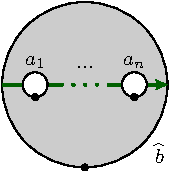
\includegraphics[]{pic-disc-standard.pdf}
\end{center}

Each standard surface comes with a collection of
\emph{standard POP decompositions}:
these will be POP decompositions where we require each
observable to cross the
equator twice and have counterclockwise orientation.
Up to isotopy, a given standard surface will have only finitely many of these.
On a standard surface with three
interior holes there are two standard POP decompositions,
and one $F$-move that relates these.
On a standard surface with four interior holes there are five 
standard POP decompositions and five $F$-moves that relate these.
In this case the $F$-moves themselves satisfy an equation
that is enforced by the axioms of the modular functor.
This is known as the pentagon equation, which we depict as
the following commutative diagram:
\begin{center}
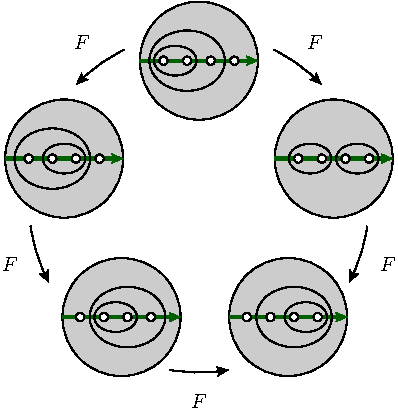
\includegraphics[]{pic-pentagon.pdf}
\end{center}

We define the vector spaces 
$ V^{a_1...a_n}_{b} := \F(\StdM).$ 
We now choose a basis for each of the
%$V^{ab}_c$ to be $\{v^{ab}_{c,\mu}\}_{\mu}.$
%$V^{a'_1a'_2}_{b'}$ to be $\{v^{a'_1a'_2}_{b',\mu}\}_{\mu}.$
$V^{a_1a_2}_{b}$ to be $\{v^{a_1a_2}_{b,\mu}\}_{\mu}.$
For every standard POP decomposition of $\StdM,$
we get a decomposition of 
$V^{a_1...a_n}_{b}$ into direct sums of various %$V^{a'b'}_{c'}.$
$V^{a'_1a'_2}_{b'}.$ 
This then gives a \emph{standard basis} of $V^{a_1...a_n}_{b}$
relative to this standard POP decomposition
using the corresponding  $\{v^{a'_1a'_2}_{b',\mu}\}_{\mu}$
for each of the $V^{a'_1a'_2}_{b'}.$ % $V^{a'b'}_{c'}.$
\simon{...ugh}

Note that for any standard surface $\StdM$ 
and any choice of $k$ contiguous holes $a_j,...,a_{j+k-1}$
we can find an observable that encloses exactly these holes
in at least one of the standard POP decompositions of $\StdM.$ 

Gluing of two standard surfaces is not in general going to
produce another standard surface. However, we can ... \simon{fix this}

\subsub{Curve diagram.}
We next study maps from standard surfaces to arbitrary surfaces.
The set of all maps from $\StdM$ 
to a surface $N$ will be denoted as $\Hom(\StdM, N).$ 
We call each such map a \emph{curve diagram},
or more specifically, a curve diagram on $N$.
The reason for this terminology is that we can reconstruct (up to isotopy)
any map $f:\StdM\to N$ from
the restriction of $f$ to the equator of $\StdM.$ 
In other words, we can uniquely specify any map
$f:\StdM\to N$ by indicating the action of
$f$ on the equator. We take full advantage of this
fact in our notation: any figure of a surface
with a ``green line'' drawn therein is actually notating a 
diffeomorphism, not a surface!

Any curve diagram will act on a standard POP decomposition
of $\StdM$ sending it to a POP decomposition of $N.$
Surprisingly, the converse of this statement also holds:
any POP decomposition of $N$ comes from some curve diagram
acting on a standard POP decomposition.
\cggb{This is true for any $N$ that is homeomorphic to a punctured disc?}
\simon{Right, I should be more clear about when exactly we specialize to discs.}
The proof of this is constructive, and we call this
the refactoring theorem below.
%The proof of this is constructive and forms the heart of
%our algorithm below.

\simon{show how to glue two curve diagrams together to get another
curve diagram}

%Any curve diagram will send a standard POP decomposition
%of $\StdM$ to a POP decompositions of $N,$ and therefore
%(via $\F$) will also send the standard basis to a basis
%of $\F(N).$
%This is how to understand the sense in which a curve diagram 
%(together with a standard POP decomposition) 
%``picks out'' a basis of $\F(N).$
%Remarkably, the converse of this result also obtains

We note in passing two connections to the mathematical literature.
Such curve diagrams have been 
used in the study of braid groups \cite{Dehornoy2002}, and this
is where the name comes from, although our
curve diagrams respect the base points and so could be further
qualified as ``framed'' curve diagrams.
And, we note the similarity of curve diagrams and associated
modular functor 
to the definition of a planar algebra \cite{Jones1999},
the main difference being that planar algebras allow for 
not just two but any even number of curve intersections at each hole.


\subsub{Z-move.}
We let $z$ be a diffeomorphism of standard surfaces 
$z : M^{a_1...a_n}_{b} \to  M^{a_2...a_n{b}}_{{a_1}}$
that preserves the equator.
(Considering the standard surface as a sphere with holes
placed uniformly around a great circle, $z$ is seen to
be a ``rotation''.)
This acts by pre-composition to
send a curve diagram $f\in \Hom(\StdM, N)$ to 
$fz \in \Hom(M^{a_2...a_n{b}}_{{a_1}}, N).$
This we call a $Z$-move of $f.$

In this way, any curve diagram can be seen as another
curve diagram that has a cyclic permutation of the labels of
the underlying standard surface.

\subsub{R-move.}
%This is a (collection of) linear operator(s)
Given anyon labels $a, b$ and $c$, and arbitrary
surface $N,$
we now define the following map of curve diagrams on $N:$
$$R^{ab}_c: \Hom(M^{ab}_c, N)\to \Hom(M^{ba}_c, N).$$
%\simon{do we need to restrict the term ``map'' as only applying to maps of surfaces?}
This map works by taking a curve diagram 
$f:M^{ab}_c\to N$ to the composition $f\sigma$ where
$\sigma:M^{ba}_c\to M^{ab}_c$
is a counterclockwise ``half-twist'' map that exchanges
the $a$ and $b$ holes.
Here we show the action of $R^{ab}_c$ on one particular curve diagram:
\begin{center}
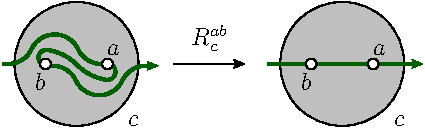
\includegraphics[]{pic-rmove-1.pdf}
\end{center}
Such an application of $R^{ab}_c$ to a particular
curve diagram we call an \emph{R-move.}
\cggb{Should the $a$ and $b$ labels be swapped on the second diagram?}
\simon{No. This is quite tricky and took me months to work out (ouch) so take care...}

%\simon{Extend $R$-move under gluing.}
As we extended Dehn twists under gluing,
we can do this for $R$-moves.
Given any pair-of-pants in $M$ ... \simon{keep going}

\simon{When do we start confusing the distinction between
topological operations and the corresponding vector space
operation via $\F$ ?}

\subsub{Skeins.}
The preivious figure can be seen as a ``top-down'' view of the
following three dimensional arrangement:
%At this point we can show the relation to skein theory:
\begin{center}
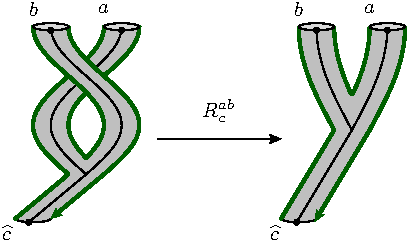
\includegraphics[]{pic-rmove-skein.pdf}
\end{center}
This figure is intended to be topologically
the same as the previous flat figure,
with the addition of a third dimension,
and the $c$ boundary has been shrunk.
Also note thin black lines
connecting the base points.
The black lines do not add any extra structure, they can
be seen as a part of the hexagon cut out by
the green line and boundary components.
But notice this: the black lines are ``framed'' by the green lines. 
These are the ribbons used in skein theory!
Note that all the holes are created equal: there is
no distinction between ``input'' holes and ``output'' holes
(as there is with cobordisms or string diagrams.)

%We can get monodromy operators, and theta operators...
%\begin{center}
%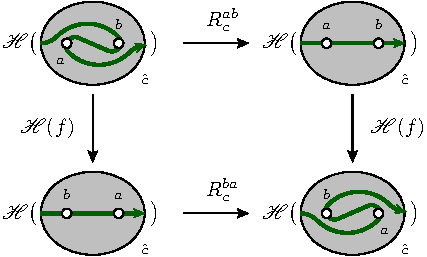
\includegraphics[]{pic-natural.pdf}
%\end{center}
%However, such a natural transform would be notated as 
%%category theorists would write this as
%$ R^{ab}_c : \F\to\F,$
%and this looks good because natural transformations
%can be thought of as $2-$morphisms (a morphism of morphisms) and we
%do expect the braiding to be somehow one level up
%in the $n-$categorical sense.

\subsub{Hexagon equation.}
For a surface with three interior holes there are
infinitely many POP decompositions (up to isotopy).
These are all made by choosing an observable 
that encloses two holes.
The $F$-moves allow us to switch between 
these POP decompositions,
and the axioms for the modular
functor make these consistent.
Here we show two such triangle consistency requirements
(they are reflections of each other):
\begin{center}
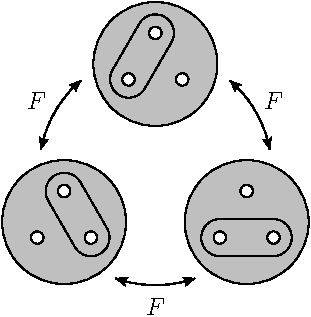
\includegraphics[width=0.25\columnwidth]{pic-fmove-relation.pdf}
\ \ \ \ \ \ \ \ \ \ \ \ \ 
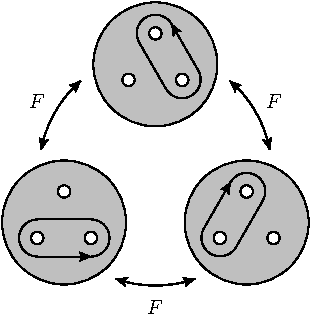
\includegraphics[width=0.25\columnwidth]{pic-fmove-relation-r.pdf}
\end{center}
Given a POP decomposition of a surface $N$
there are various curve diagrams on $N$ that
produce this decomposition from 
a standard POP decomposition, and there are certain $R$-moves
will map between these.
Once again, these moves must be consistent, and
here we note the two ``hexagon equations'' 
%for curve diagrams corresponding to the above triangles:
corresponding to the above two triangles:
\begin{center}
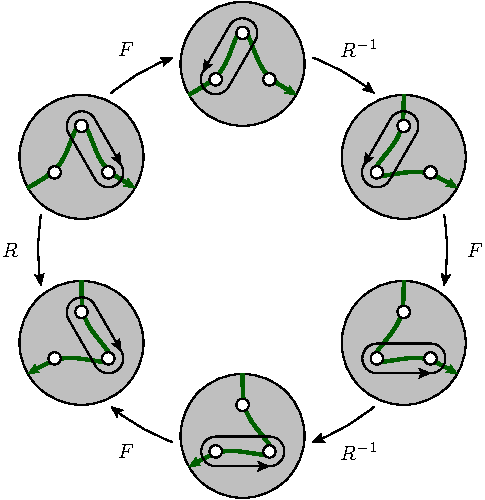
\includegraphics[width=0.4\columnwidth]{pic-hexagon.pdf}
\ \ \ \ \ \ \ \ \ \ \ \ 
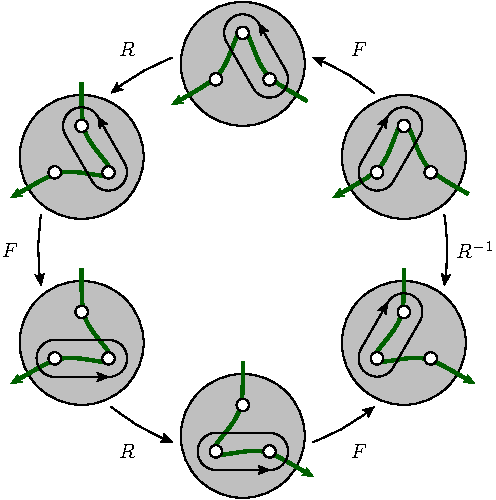
\includegraphics[width=0.4\columnwidth]{pic-hexagon-r.pdf}
\end{center}
Note that we have neglected to indicate the base points here.
Given a curve diagram, we can agree that base points
occur ``to the right'' of the image of the equator.
But in notating diagrams such as these, there is still
an ambiguity: the position of the base points should be the
same in each surface in the diagram.
If we try to correct for this post-hoc
by rotating individual holes,
we will then be correct
only up to possible Dehn twist(s) around each hole.
We can certainly track these twists if we wanted to,
but in the interests of simplicity we do not.
This introduces a global phase ambiguity into the
calculations.
%What we have done here is to forget that the holes
%have width, and shrunk them to points.

\section{Refactoring theorem}

In this section we specialize to considering planar 
surfaces only.
The theorem we are building towards shows that
the $R$-moves act transitively on curve diagrams.
\simon{We don't much care about transitivity. Should specialize this.}
That is, given two curve diagrams $f$ and $f'$ on $N$ we can find
a sequence of $R$-moves that transform $f$ to $f'.$
%We consider surface $N$ with $n$ boundary components
%$a_1,...,a_n.$
The key idea is to consider the (directed) image of the equator under
%the curve diagrams $f$ and $f'$.
these curve diagrams.
As mentioned previously, this image is sufficient to
define the entire diffeomorphism (up to isotopy) and so we are free
to work with just this image, or \emph{curve},
and we confuse the distinction between 
a curve diagram (a diffeomorphism)
and its curve.
%which we refer to as a \emph{curve.}
%Each such image will touch all the holes of $N.$

The construction proceeds by considering adjacent
pairs of holes along $f'$ and then acting on the
portion of $f$ between these same two holes so that
they then become adjacent on the resulting curve.
Continuing this
process for each two adjacent holes of $f'$ will then
show a sequence of $R$-moves that sends $f$ to $f'.$
\simon{still not obvious: what if some such $R$-move
destroys a previously adjacentized pair of holes?}

To this end, consider a sequence of holes $a_1,...,a_n$
appearing sequentially along $f$
such that $a_1$ and $a_n$ appear sequentially on $f'.$
We may need to apply some $Z$-moves to $f$ to ensure
that $a_1$ appears sequentially before $a_n$.
Now consider the case such that
along $f'$ between these two holes there is
no intersection with $f.$
We form a closed path $\xi$ by
following the $f'$ curve between $a_1$ and $a_n$ and then
following the $f$ curve in reverse from $a_n$ back to $a_1.$
(Note that to be completely rigorous here we would need to include segments
of path contained within boundary components.)
The resulting closed path bounds a disc.
If $\xi$ has clockwise orientation \simon{XX define clockwise XX}
we apply the following sequence of $R$-moves to $f$:
$$
    R^{a_1a_2}_{b_1}, R^{a_1a_3}_{b_2}, ..., R^{a_1a_{n-1}}_{b_{n-1}}.
$$
Depicted here is the first such move:
\begin{center}
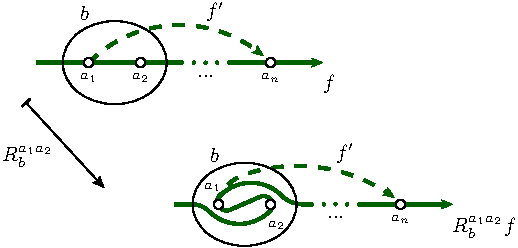
\includegraphics[]{pic-theorem.pdf}
\end{center}
After each of these $R$-moves the closed path
formed by 
following the $f'$ curve between $a_1$ and $a_n$ and then
following the $R$-moved $f$ curve back to $a_1$ will
traverse one less hole, and still bound a disc.
After all of the $R$-moves this path will only
touch $a_1$ and $a_n,$ and bound a disc.
Therefore, we have acted on the $f$ curve so that
the resulting curve has $a_1$ and $a_n$ adjacent
and the bounded disc gives an isotopy for that
segment of the curve.

When the closed curve $\xi$ has anti-clockwise orientation
we use the same sequence of $R$-moves but with $R$ replaced by $R^{-1}.$

Generalizing further,
when the $f'$ curve between $a_1$ and $a_n$ has (transverse) intersections
with $f$ we use every such intersection to indicate a switch
between using $R$ and $R^{-1}.$

%\simon{what if the direction of $f$ is reversed??
%eg. $f$ and $f'$ are the same except one has reverse direction?}

This refactoring theorem will be reformulated 
below as a combinatorial ``paperclip algorithm''.

\simon{Use $c$ instead of $f$ for curve diagrams?}

%
% ~~~~~~~~~~~~~~~~~~~~~~~~~~~~~~~~~~~~~~~~~~~~~~~~~~~~~~~~~~~~~~~~~~~~~~~~~~~~
%

\section{Physical model}

The manifold underlying our system is a torus.
We endow this with a $L\times L$ square lattice of observables:
$$
    \Lambda := \bigl\{ \gamma_{ij} \bigr\}_{i,j=1,...,L}
$$
These observables are the physically accessible observables of
the noise reduction procedure we call the \emph{decoder.}
We call each such $\gamma_{ij}$ a \emph{tile.}
We show a small gap between the tiles but this is not meant
to reflect an actual physical gap.

The noise process acts to populate the manifold with
a randomly distributed set of pair creation processes,
whose size is much smaller than the resolution of the lattice.
We model this as a random distribution of pair-of-pants:
\begin{center}
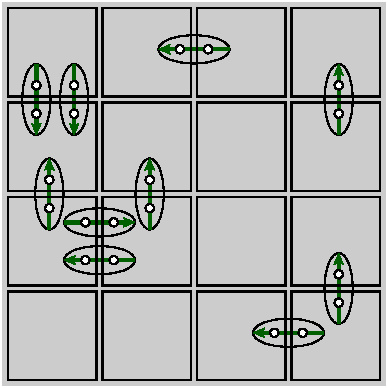
\includegraphics[]{pic-pair-create.pdf}
\end{center}

Each such pair will have vacuum total charge and so the observables
$\gamma_{ij}$ will only see pairs that intersect, ie. we
need only consider distributing these pairs
transversally along edges of the tiles.

In order to compute measurement outcomes for the $\gamma_{ij}$
we first need to concatenate any two curve diagrams that 
participate in the same $\gamma_{ij}.$
Because each curve has vacuum total charge this can be
done in an arbitrary way:
\begin{center}
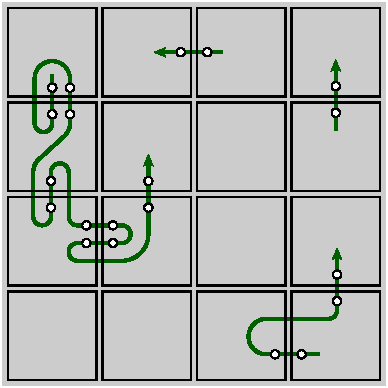
\includegraphics[]{pic-join-pairs.pdf}
\end{center}

Working in the basis picked out by the resulting curve
diagrams, we can calculate measurement outcomes for each tile,
the result of which is recorded on the original curve:
\begin{center}
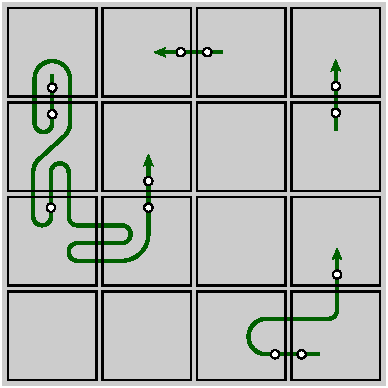
\includegraphics[]{pic-curve-uniq.pdf}
\end{center}
\cggb{It might be helpful to be a bit more explicit either here or later about exactly how we perform this step, moving charges around with the paperclip algorithm until they are all neighbouring and then we are in a standard basis and can use F-moves to calculate fusion outcomes.}
\simon{good idea}


%The details of how this is implemented computationally,
%the data structures and algorithm, we have not yet described
%and this is what we turn to next.

%
% ~~~~~~~~~~~~~~~~~~~~~~~~~~~~~~~~~~~~~~~~~~~~~~~~~~~~~~~~~~~~~~~~~~~~~~~~~~~~
%

%
% ~~~~~~~~~~~~~~~~~~~~~~~~~~~~~~~~~~~~~~~~~~~~~~~~~~~~~~~~~~~~~~~~~~~~~~~~~~~~
%

%\section{The refactoring theorem}
%
%
%  XXX useless
%\begin{center}
%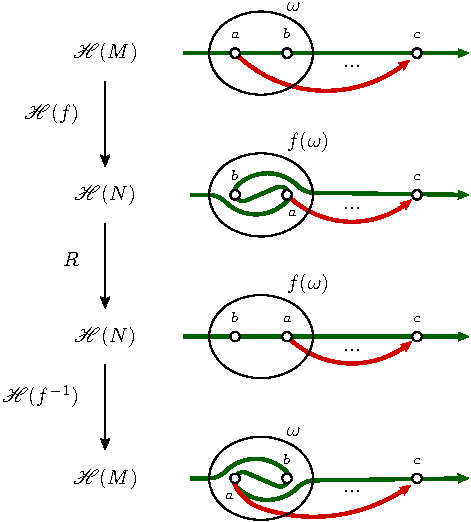
\includegraphics[]{pic-refactoring.pdf}
%\end{center}

%
% ~~~~~~~~~~~~~~~~~~~~~~~~~~~~~~~~~~~~~~~~~~~~~~~~~~~~~~~~~~~~~~~~~~~~~~~~~~~~
%

\section{Combinatorial curve diagrams}

The basic data structure involved in the
simulation we term a \emph{combinatorial curve diagram.}
% XXX define "piece of curve"
Firstly, we will require each curve to intersect 
the edges of tiles transversally,
and in particular a curve will not touch a tile corner.

For each tile in the lattice,
we store a combinatorial
description of the curve(s) intersected with that tile.
Each component of such an intersection we call a \emph{piece-of-curve.}
\begin{center}
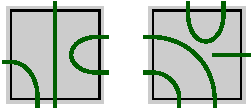
\includegraphics[]{pic-cells.pdf}
\end{center}

We follow essentially the same approach as taken in \cite{Abramsky2007} 
to describe elements of a Temperley-Leib algebra, but
with some extra decorations.
The key idea is to store a \emph{word} for each tile, comprised of
the letters $\bigl<$ and $\bigr>$.
%The encoding works as follows.
Reading in a clockwise direction around the edge of
the tile from the top-left corner,
we record our encounters with each piece-of-curve,
writing~$\bigl<$ for the first encounter, and~$\bigr>$ for the
second.
We may also encounter a dangling piece-of-curve
(the head or the tail), so we use another symbol $*$ for this.
The words for the above two tiles will then be 
$\bigl<\bigl<\bigr>\bigr>\bigl<\bigr>$ and $\bigl<\bigr>*\bigl<\bigl<\bigr>\bigr>.$
When the brackets are balanced,
each such word will correspond one-to-one with an intersection
of a curve in a tile, up to a continuous deformation of the interior of the tile.
Ie. the data structure 
will be insensitive to any continuous deformation of the interior of the tile,
but the simulation does not need to track any of these degrees of freedom.

\begin{center}
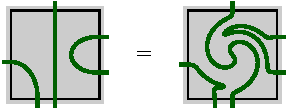
\includegraphics[]{pic-cells-0.pdf}
\end{center}

We will also need to record
various other attributes of these curves,
and to do this we make this notation more elaborate
in the paragraphs {\bf (I)}, {\bf(II)} and {\bf(III)} below.
Each symbol in the word describes an intersection of
the curve with the tile boundary,
and so as we decorate these symbols these decorations will
apply to such intersection points.

\begin{center}
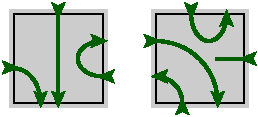
\includegraphics[]{pic-cells-1.pdf}
\end{center}

{\bf (I)} We will record the direction of each piece-of-curve,
this will be either an {\tt in} or {\tt out} decoration for each symbol.
Such decorations need to balance according to the brackets.
The decorated symbols $*_{\mbox{\tt in}}$ and 
$*_{\mbox{\tt out}}$ 
will denote respectively either
%the head, $c(1)$ or the tail $c(0)$ of a curve.
the head or the tail of a curve.
The words for the diagrams above now read as
$ \bigl<_{\mbox{\tt in}}\bigl<_{\mbox{\tt out}}\bigr>_{\mbox{\tt in}}
    \bigr>_{\mbox{\tt out}}\bigl<_{\mbox{\tt out}}\bigr>_{\mbox{\tt in}}$
and
$ \bigl<_{\mbox{\tt in}}\bigl>_{\mbox{\tt out}}*_{\mbox{\tt in}}
    \bigr<_{\mbox{\tt out}}
    \bigr<_{\mbox{\tt in}}\bigl>_{\mbox{\tt out}}\bigr>_{\mbox{\tt in}}.
$

{\bf (II)} We will record,
for each intersection with the tile edge, 
a numeral indicating which of the four
sides of the tile the
intersection occurs on.
Numbering these clockwise from the top as $1, 2, 3, 4$ we have for the above curves: 
$\bigl<_1\bigl<_2\bigr>_2\bigr>_3\bigl<_3\bigr>_4$ 
and $\bigl<_1\bigr>_1*_2\bigl<_3\bigl<_3\bigr>_4\bigr>_4.$

{\bf (III)} Finally, we will also decorate these symbols with anyons.
This will be an index to a leaf of a (sum of) fusion tree(s).
This means that anyons only reside on the curve close
to the tile boundary,
and so we cannot have more than two anyons
for each piece-of-curve. 
The number of such pieces is arbitrary, and so this
is no restriction on generality.

\begin{center}
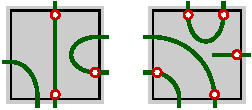
\includegraphics[]{pic-cells-2.pdf}
\end{center}

In joining tiles together to make a tiling we will
require adjacent tiles to agree on their shared boundary.
This will entail sequentially pairing symbols in the
words for adjacent tiles
and requiring that 
the {\tt in} and {\tt out} decorations are matched.
Because the word for a tile proceeds conter-clockwise
around the tile, this pairing will always reverse the
sequential order of the symbols of adjacent tiles.
For example, given the above two tiles we sequentially pair the 
$\bigl<_{\mbox{\tt out},2}\bigr>_{\mbox{\tt in},2}$ 
and $\bigr>_{\mbox{\tt out},4}\bigr>_{\mbox{\tt in},4}$
symbols with opposite order so that
$\bigl<_{\mbox{\tt out},2}\sim\bigr>_{\mbox{\tt in},4}$
and $\bigr>_{\mbox{\tt in},2} \sim \bigr>_{\mbox{\tt out},4}.$ 

%Two other consistency relations are enforced on such a combinatorial curve diagram:
%we require adjacent tiles to agree on their boundaries, 
%and every curve diagram
%must have two ends.
%One final consistency
%relation is enforced by requiring 
%We require every curve diagram to have two ends, this means
%that there are no loops.

Note that in general this data structure will store many disjoint curve diagrams
$c_i:[0,1]\to D_{n_i}$ within a disc $D_m$ where $\sum n_i = m.$

%For a given piece-of-curve, we can subtract the numeral with
%the {\tt in} label from the numeral with the {\tt out} label
%to get an integer in $\{ \}$ WRONG
%We can also just use the numerals of the boundary edges
%that the piece-of-curve intersects with, subtracting the
%``exit'' boundary numeral from the ``entry'' boundary numeral. WRONG

For each piece-of-curve, apart from a head or tail, there is an associated 
number we call the \emph{turn number}. This counts the number
of ``right-hand turns'' the piece-of-curve makes as it
traverses the tile, with a ``left-hand turn'' counting as $-1.$
(To be more rigorous, we would define this number using the
winding number of the simple closed curve formed by the
piece-of-curve adjoined to a segment of the boundary of the tile 
traversed in a clockwise direction.)
This number will take one of the values $-2, -1, 0, 1, 2:$
\begin{center}
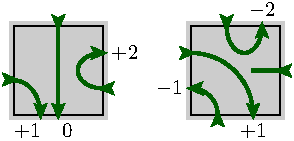
\includegraphics[]{pic-cells-3.pdf}
\end{center}


%Two disjoint curves can be joined by...
%
%Curves can be simplified along sections without any anyons, ...

% Each piece will have +1, +2, 0, -1, -2 right-hand turns...

% mention Jones' planar algebras ?

%
% ~~~~~~~~~~~~~~~~~~~~~~~~~~~~~~~~~~~~~~~~~~~~~~~~~~~~~~~~~~~~~~~~~~~~~~~~~~~~
%

\section{The paperclip algorithm}

Anyons are transported around the lattice
by moving them along tile edges.
\simon{Note that transport here is the same as the refactoring from above.}
In general, such a transport will intersect with a
curve diagram in many places.
Each such intersection is transverse,
and we use each intersection point to cut
the entire transport into smaller paths each of
which touch the curve diagram twice.
%Each intersection with a curve diagram
%will then be transverse, and we
%decompose the entire path into a sequence of
%paths each of which 
%join consecutive intersections.
%Transport of an anyon can be decomposed into
%moves between adjacent components of a curve
%diagram.
The origin and destination of such an anyon path
now splits the curve diagram $c:[0, 1]\to D_n$ 
into three disjoint pieces which we term
\emph{head}, \emph{body} and \emph{tail}, where
the head contains the point $c(1)$, the tail
contains $c(0)$ and the body is the third piece.
These arise with various arrangements, but here
we focus on one instructive case, the
other cases are similar:
%We look at the particular case of moving along
%one edge of a tile,
transporting along one edge of a tile \emph{forwards} 
(from tail to head) along a curve diagram:
\begin{center}
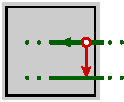
\includegraphics[]{pic-move-anyon.pdf}
\end{center}

This arrangement is equivalent (isotopic) to one of four 
``paperclips'', which we distinguish between by counting how
many \emph{right-hand turns} are made along the body of the curve diagram.
We also show an equivalent (isotopic) picture where the
curve diagram has been straightened, and the resulting distortion
in the anyon path:
\begin{center}
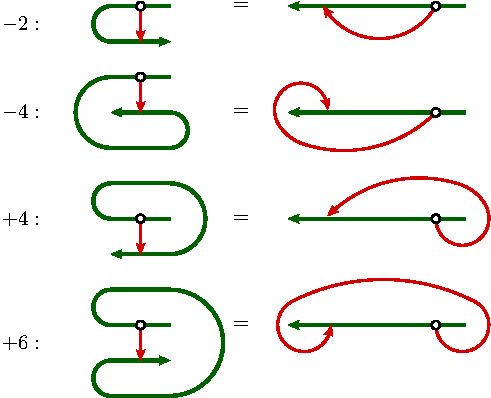
\includegraphics[]{pic-paperclip.pdf}
\end{center}
The sequence of anyons along the head, body and tail, we denote as $H, B$ and $T,$
respectively.
These sequences have the same order as the underlying curve diagram, and 
we use
$H^r, B^r$ and $T^r$ to denote the same anyons with the reversed order.
Using the above diagram, we can now read off the $R$-moves for each
of the four paperclips:
\begin{align*}
-2:&\ R[B] \\
-4:&\ R[H^r]\ R[H]\ R[B] \\
+4:&\ R[B]\ R[T]\ R[T^r] \\
+6:&\ R[H^r]\ R[H]\ R[B]\ R[T]\ R[T^r] \\
\end{align*}
where notation such as $R[B]$ is understood as sequentially clockwise braiding around
each anyon in $B$.

That these four paperclips exhaust all possibilities can be seen by
considering the winding number of the simple closed curve made
by combining the body of the curve diagram with the path followed by
the anyon (appropriately reversing direction as needed).

%
% ~~~~~~~~~~~~~~~~~~~~~~~~~~~~~~~~~~~~~~~~~~~~~~~~~~~~~~~~~~~~~~~~~~~~~~~~~~~~
%

\section{Decoding algorithm}

After the noise process is applied to the system,
the error correction proceeds as a dialogue between the
decoder and the system. 
The decoder measures succesively larger and larger
regions of the lattice
until there are no more charges 
or a topologically non-trivial operation has occured
(an operation that spans the entire lattice.)
Here we show this in a process diagram, with time running up
the page:
\begin{center}
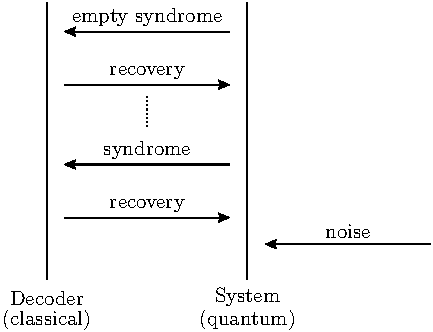
\includegraphics[]{pic-process.pdf}
\end{center}

So far we have discussed the simulation of the (quantum) system
and now we turn to the decoder algorithm.
Here is a pseudo-code listing for this,
and we explain each step via an example below.

\begin{verbatim}
 1:  def decode():
 2:      syndrome = get_syndrome()
 3:      
 4:      # build a cluster for each charge
 5:      clusters = [Cluster(charge) for charge in syndrome]
 6:  
 7:      # join any neighbouring clusters
 8:      join(clusters, 1)
 9:      
10:      while clusters:
11:      
12:          # find total charge on each cluster
13:          for cluster in clusters:
14:              fuse_cluster(cluster)
15:      
16:          # discard vacuum clusters
17:          clusters = [cluster for cluster in clusters if non_vacuum(cluster)]
18:      
19:          # grow each cluster by 1 unit
20:          for cluster in clusters:
21:              grow_cluster(cluster, 1)
22:      
23:          # join any intersecting clusters
24:          join(clusters, 0)
25:  
26:      # success !
27:      return True
\end{verbatim} % see decode.py

First, we show the result of the initial call to {\tt get\_syndrome()}, on line 2.
The locations of anyon charges are highlighted in red.
For each of these charges we build a {\tt Cluster}, on line 5.
Each cluster is shown as a gray shaded area.
\begin{center}
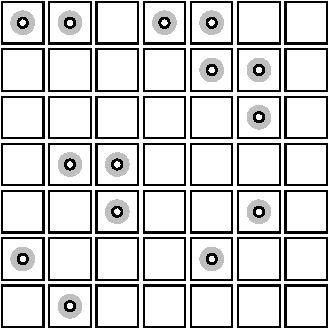
\includegraphics[]{pic-decode-0.pdf}
\end{center}
The next step is the call to {\tt join(clusters, 1)}, on line 8,
which joins clusters that are separated by at most one lattice
spacing. We now have seven clusters:
\begin{center}
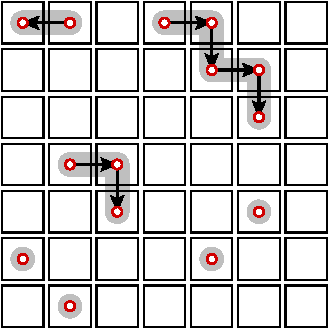
\includegraphics[]{pic-decode-1.pdf}
\end{center}
Each cluster is structured as a rooted tree, as indicated by
the arrows which point in the direction from the leaves to
the root of the tree. 
This tree structure is used in the call to {\tt fuse\_cluster()},
on line 14.
This moves anyons in the tree along the arrows to the root, 
fusing with the charge at the root.
\begin{center}
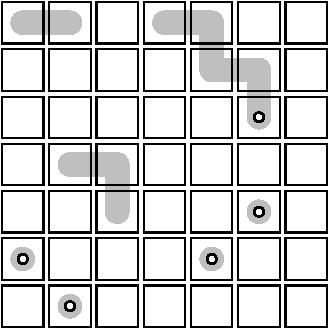
\includegraphics[]{pic-decode-2.pdf}
\end{center}
For each cluster, the resulting charge at the root is taken as the charge of
that cluster. Any cluster with vacuum total charge is then discarded (line 17).
%In our example, we assume all these charges are non-vacuum.
In our example, we find two clusters with vacuum charge and we discard these.
The next step is to grow the remaining clusters by one lattice spacing (line 20-21),
and join (merge) any overlapping clusters (line 24).
\begin{center}
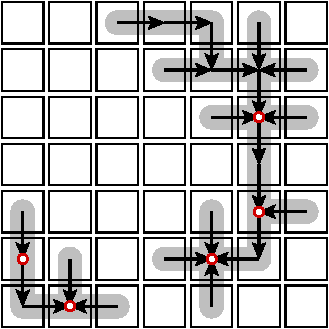
\includegraphics[]{pic-decode-3.pdf}
\end{center}
%Now we are down to two clusters.
Note that we can choose the root of each cluster arbitrarily,
as we are only interested in the total charge of each cluster.

We repeat these steps of fusing, growing and then joining clusters (lines 10-24.)
If at any point this causes a topologically 
non-trivial operation, the simulation aborts and a failure
to decode is recorded.
Otherwise we eventually run out
of non-vacuum clusters, and the decoder succeeds (line 27).
Note that for simplicity we have neglected the boundary of the lattice in
this example.

\cggb{Maybe it is worthwhile to briefly recall the broad structure of our simulation somewhere here to help structure the discussion. I.e.~we have first noise creation, then we iterate \{syndrome measurement, classical decoding algorithm, transport\} until failure or success.}
\simon{I agree the structure needs work.}

%\section{Computation of homologically non-trivial operators}\label{s:homnontrivial}
%
%Specializing to the Fibonacci case,
%we write the non-trivial $F$-moves as the following
%skein relations:
%\begin{align*}
%\includegraphics[]{pic-skein1.pdf}
%\end{align*}
%
%The sollid lines represent Fibonacci world-lines.
%The dotted lines represent vacuum charges,
%and we are free to include these lines or not.
%We leave these anyon paths
%as undirected because Fibonacci anyons are
%self-inverse.
%The non-trivial $R$-moves are:
%\begin{align*}
%\includegraphics[]{pic-skein2.pdf}
%\end{align*}
%
%Removing bubbles:
%\begin{align*}
%\includegraphics[]{pic-bubble.pdf}
%\end{align*}
%
%Here we show a process where a 
%Fibonacci anyon travels around the torus and
%anihilates itself. Twice.
%The vertical lines represent a periodic
%identification.
%\begin{align*}
%\includegraphics[]{pic-logops.pdf}
%\end{align*}
%
%The state is not normalized.
%Also involves post-selection, as there is
%another process that involves leakage...
%The first equation is an $F$-move, 
%the second equation is a translation in the
%horizontal direction, and the last equation
%follows from the rule for collapsing bubbles.
%
%Continuing in this way, we compute the $k$-fold
%logical operator:
%\begin{align*}
%\includegraphics[]{pic-kfold.pdf}
%\end{align*}
%
%where $f_k$ is the $k$-th element of the Fibonacci
%sequence $\{1, 1, 2, 3...\}.$

% CUT HERE

%------------------------------------------------------------------------------------------------------------%
\bibliography{refs2}



\end{document}
